%=============================================================
%  BEAMER PRESENTATION - INTRODUCTION + RELATED WORKS
%  Gán nhãn bằng LLM có kiểm chứng cho dữ liệu tiếng Việt
%  Ý định thương mại điện tử phân cấp
%=============================================================
\documentclass[10pt,aspectratio=169]{beamer}
\usepackage[utf8]{vietnam}
\usepackage{amsmath,amssymb,amsfonts}
\usepackage{booktabs,array,longtable}
\usepackage{graphicx}
\usepackage{tikz}
\usetikzlibrary{shapes,arrows,arrows.meta,positioning,calc,
                shapes.geometric,fit,decorations.pathreplacing,
                decorations.markings,backgrounds,shadows}
\usepackage{pgfplots}
\pgfplotsset{compat=1.18}
\usepackage[many]{tcolorbox}
\usepackage{fontawesome5}
% Fallback cho icon không có trong fontawesome5 free (Overleaf)
\makeatletter
\@ifundefined{faShield}{\newcommand{\faShield}{\faCheckCircle}}{}
\@ifundefined{faShieldAlt}{\newcommand{\faShieldAlt}{\faCheckCircle}}{}
\@ifundefined{faLayerGroup}{\newcommand{\faLayerGroup}{\faCubes}}{}
\@ifundefined{faProjectDiagram}{\newcommand{\faProjectDiagram}{\faSitemap}}{}
\makeatother
\usepackage{hyperref}

%=============================================================
%  1. TEMPLATE CUSTOMIZATION
%=============================================================
\definecolor{uitblue}{RGB}{108,79,59}
\definecolor{uitdark}{RGB}{74,53,37}
\definecolor{accent}{RGB}{197,140,50}
\definecolor{accentlt}{RGB}{222,178,110}
\definecolor{greenteal}{RGB}{100,120,80}
\definecolor{lightgray}{RGB}{248,245,240}
\definecolor{textgray}{RGB}{60,55,50}

% Beamer đã nạp hyperref; chỉ cấu hình, tránh option clash.
\hypersetup{colorlinks=true,linkcolor=uitblue,urlcolor=uitblue,citecolor=uitblue}

% Các file ảnh cần nằm cùng thư mục với file .tex.
% Nếu file không tồn tại, template sẽ tự bỏ qua ảnh tương ứng.
\newcommand{\titlebgimage}{title_bg.png}
\newcommand{\sectionbgimage}{section_bg.png}
\newcommand{\logonhomNC}{logo_nhom_nc.png}
\newcommand{\logonhomthuchien}{logo_nhom_thuchien.png}
\newcommand{\gvhd}{PGS.TS Nguyễn Đình Thuân, ThS. Đỗ Duy Thanh}
\newcommand{\slidewatermark}{logo_nhom_nc.png}
\newcommand{\contactemail}{ftisu@uit.edu.vn}

%=============================================================
%  2. THÔNG TIN BÁO CÁO
%=============================================================
\title[Mở rộng hierarchical intent sang banking]
{Mở rộng Hierarchical Intent Annotation từ Vietnamese E-commerce sang Banking Domain}
\subtitle{Báo cáo tiến độ nghiên cứu Master về NLP: xây dựng taxonomy cho BANKING77}
\author{Nguyễn Huỳnh Minh Huy}
\date{05/10/2026}

%=============================================================
%  3. BEAMER THEME OVERRIDE
%=============================================================
\usetheme{default}
\usecolortheme{default}
\setbeamertemplate{navigation symbols}{}

\setbeamercolor{palette primary}{bg=uitblue,fg=white}
\setbeamercolor{frametitle}{bg=uitblue,fg=white}
\setbeamercolor{title}{bg=uitblue,fg=white}
\setbeamercolor{author in head/foot}{bg=uitdark,fg=white}
\setbeamercolor{title in head/foot}{bg=uitblue,fg=white}
\setbeamercolor{date in head/foot}{bg=uitdark!80,fg=white}
\setbeamercolor{section in head/foot}{bg=uitblue!70,fg=white}
\setbeamercolor{block title}{bg=uitblue!18,fg=uitdark}
\setbeamercolor{block body}{bg=uitblue!5,fg=textgray}
\setbeamercolor{alertblock title}{bg=accent!20,fg=accent!80!black}
\setbeamercolor{alertblock body}{bg=accent!5,fg=textgray}
\setbeamercolor{exampleblock title}{bg=greenteal!20,fg=greenteal!70!black}
\setbeamercolor{exampleblock body}{bg=greenteal!5,fg=textgray}
\setbeamercolor{item}{fg=uitblue}
\setbeamercolor{subitem}{fg=accent}
\setbeamercolor{enumerate item}{fg=uitblue}
\setbeamercolor{normal text}{fg=textgray}
\setbeamercolor{structure}{fg=uitblue}

% Watermark: chỉ hiển thị khi file thực sự tồn tại.
\usebackgroundtemplate{
  \IfFileExists{\slidewatermark}{
    \begin{tikzpicture}[remember picture,overlay]
      \node[opacity=0.03,anchor=center] at (current page.center) {
        \includegraphics[width=0.30\paperwidth]{\slidewatermark}
      };
    \end{tikzpicture}
  }{}
}

\setbeamertemplate{frametitle}{
  \vskip2pt
  \begin{beamercolorbox}[wd=\paperwidth,ht=0.56cm,dp=0.2cm,leftskip=0.4cm]{frametitle}
    \usebeamerfont{frametitle}\insertframetitle
    \ifx\insertframesubtitle\empty\else
      \;{\small\textcolor{accentlt}{$\triangleright$}}\;\usebeamerfont{framesubtitle}\textcolor{accentlt}{\insertframesubtitle}
    \fi
  \end{beamercolorbox}
  \vskip-2pt
  \begin{beamercolorbox}[wd=\paperwidth,ht=1.2pt,dp=0pt]{palette primary}
    \color{accent}\rule{\paperwidth}{1.2pt}
  \end{beamercolorbox}
}

\setbeamertemplate{footline}{
  \begin{beamercolorbox}[wd=\paperwidth,ht=0.4cm,dp=0.12cm]{author in head/foot}
    \hspace{0.3cm}{\scriptsize\faUniversity\; UIT -- Khoa Hệ thống Thông tin}
    \hfill
    {\scriptsize Báo cáo khoa học}
    \hfill
    {\scriptsize\insertframenumber/\inserttotalframenumber\hspace{0.3cm}}
  \end{beamercolorbox}
}

\setbeamertemplate{headline}{
  \begin{beamercolorbox}[wd=\paperwidth,ht=0.06cm]{section in head/foot}
    \color{accent}\rule{\paperwidth}{0.06cm}
  \end{beamercolorbox}
}

\setbeamertemplate{itemize item}{\color{uitblue}{\faCircle[regular]}}
\setbeamertemplate{itemize subitem}{\color{accent}$\triangleright$}
\setbeamertemplate{enumerate item}{\color{uitblue}\insertenumlabel.}

\setbeamertemplate{title page}{
  \begin{tikzpicture}[remember picture,overlay]
    \fill[uitblue] (current page.north west) rectangle
      ([yshift=-0.58\paperheight]current page.north east);
    \fill[uitdark] ([yshift=-0.58\paperheight]current page.north west) rectangle
      ([yshift=-0.62\paperheight]current page.north east);
    \fill[lightgray] ([yshift=-0.62\paperheight]current page.north west) rectangle
      (current page.south east);

    % Ảnh nền bìa: chỉ hiển thị nếu file tồn tại.
    \IfFileExists{\titlebgimage}{
      \node[opacity=0.10,anchor=center,inner sep=0pt] at (current page.center) {
        \includegraphics[width=\paperwidth,height=\paperheight]{\titlebgimage}
      };
    }{}

    \node[white,anchor=north west,font=\large\bfseries,align=left,
          text width=0.9\paperwidth] (univ) at
      ([xshift=0.5cm,yshift=-0.4cm]current page.north west)
      {\faUniversity\quad TRƯỜNG ĐẠI HỌC CÔNG NGHỆ THÔNG TIN -- UIT \\
       \small\normalfont Khoa Hệ thống Thông tin $|$ Nhóm nghiên cứu FTISU};

    \node[white,anchor=north west,font=\LARGE\bfseries,
          text width=0.88\paperwidth,align=left] (title) at
      ([yshift=-0.25cm]univ.south west) {\inserttitle};

    \node[accentlt,anchor=north west,font=\normalsize\slshape,
          text width=0.88\paperwidth,align=left] (subtitle) at
      ([yshift=-0.15cm]title.south west) {\insertsubtitle};

    \node[uitdark,anchor=north west,font=\small,align=left] at
      ([xshift=0.8cm,yshift=-0.66\paperheight]current page.north west)
      {\faUser\quad \insertauthor \\
       \faGraduationCap\quad GVHD: \gvhd \\
       \faEnvelope\quad \contactemail \\
       \faCalendar\quad \insertdate};

    \draw[accent,line width=4pt]
      ([xshift=0.5cm,yshift=-0.65\paperheight]current page.north west) --
      ([xshift=0.5cm,yshift=-0.88\paperheight]current page.north west);

    % Hai logo ở góc dưới bên phải; tự bỏ qua logo bị thiếu.
    \IfFileExists{\logonhomthuchien}{
      \node[anchor=south east,inner sep=0pt] (logo2) at
        ([xshift=-0.5cm,yshift=0.4cm]current page.south east) {
          \includegraphics[height=0.7cm]{\logonhomthuchien}
        };
      \IfFileExists{\logonhomNC}{
        \node[anchor=east,inner sep=0pt] at ([xshift=-0.2cm]logo2.west) {
          \includegraphics[height=0.7cm]{\logonhomNC}
        };
      }{}
    }{
      \IfFileExists{\logonhomNC}{
        \node[anchor=south east,inner sep=0pt] at
          ([xshift=-0.5cm,yshift=0.4cm]current page.south east) {
            \includegraphics[height=0.7cm]{\logonhomNC}
          };
      }{}
    }
  \end{tikzpicture}
}

\AtBeginSection[]{
  {
    \usebackgroundtemplate{
      \begin{tikzpicture}[remember picture,overlay]
        \IfFileExists{\sectionbgimage}{
          \node[anchor=center,inner sep=0pt] at (current page.center) {
            \includegraphics[width=\paperwidth,height=\paperheight]{\sectionbgimage}
          };
        }{}
        \fill[uitblue,opacity=0.92]
          (current page.north west) rectangle (current page.south east);
      \end{tikzpicture}
    }
    \begin{frame}[plain]
      \centering
      \vspace{1.8cm}
      {\color{white}\Huge\bfseries\thesection}
      \par\vskip0.3cm
      {\color{accent}\rule{0.5\paperwidth}{2pt}}
      \par\vskip0.4cm
      {\color{accentlt}\Large\bfseries\insertsectionhead}
    \end{frame}
  }
}

%=============================================================
%  4. TCOLORBOX
%=============================================================
\tcbuselibrary{skins,breakable}

\newtcolorbox{uitbox}[2][]{
  enhanced,
  colback=uitblue!6, colframe=uitblue, coltitle=white,
  fonttitle=\bfseries\small, title={#2},
  boxrule=0.5pt, arc=4pt, left=4pt, right=4pt, top=3pt, bottom=3pt,
  attach boxed title to top left={yshift=-2mm,xshift=4mm},
  boxed title style={colback=uitblue, arc=3pt, boxrule=0pt},
  #1
}

\newtcolorbox{accentbox}[2][]{
  enhanced,
  colback=accent!6, colframe=accent, coltitle=white,
  fonttitle=\bfseries\small, title={#2},
  boxrule=0.5pt, arc=4pt, left=4pt, right=4pt, top=3pt, bottom=3pt,
  attach boxed title to top left={yshift=-2mm,xshift=4mm},
  boxed title style={colback=accent, arc=3pt, boxrule=0pt},
  #1
}

\newtcolorbox{greenbox}[2][]{
  enhanced,
  colback=greenteal!6, colframe=greenteal, coltitle=white,
  fonttitle=\bfseries\small, title={#2},
  boxrule=0.5pt, arc=4pt, left=4pt, right=4pt, top=3pt, bottom=3pt,
  attach boxed title to top left={yshift=-2mm,xshift=4mm},
  boxed title style={colback=greenteal, arc=3pt, boxrule=0pt},
  #1
}

\newtcolorbox{orangebox}[2][]{
  enhanced,
  colback=accent!10, colframe=accent!85!black, coltitle=white,
  fonttitle=\bfseries\small, title={#2},
  boxrule=0.5pt, arc=4pt, left=4pt, right=4pt, top=3pt, bottom=3pt,
  attach boxed title to top left={yshift=-2mm,xshift=4mm},
  boxed title style={colback=accent!85!black, arc=3pt, boxrule=0pt},
  #1
}

\newcommand{\highlight}[1]{\textcolor{accent}{\bfseries #1}}
\newcommand{\kw}[1]{\textcolor{uitblue}{\bfseries #1}}

% Ảnh minh họa: không làm fail compile nếu file chưa có trong project Overleaf.
\newcommand{\safeincludegraphics}[2][]{%
  \IfFileExists{#2}{%
    \includegraphics[#1]{#2}%
  }{%
    \fcolorbox{uitblue!35}{uitblue!6}{%
      \parbox{0.88\linewidth}{\centering\vspace{0.35cm}
        {\scriptsize Không tìm thấy ảnh}\\[2pt]
        {\tiny\texttt{\detokenize{#2}}}
        \vspace{0.35cm}}%
    }%
  }%
}

%=============================================================
%  PHẦN THÂN
%=============================================================
\tikzset{
  stage/.style={draw=uitblue,fill=uitblue!6,rounded corners=3pt,
    minimum height=0.65cm,text width=2.8cm,align=center,font=\small},
  focus/.style={stage,draw=greenteal,fill=greenteal!12},
  future/.style={stage,draw=textgray!45,fill=lightgray,dashed},
  leaf/.style={draw=uitblue!30,fill=lightgray,rounded corners=2pt,
    minimum height=0.46cm,align=left,font=\scriptsize},
  link/.style={-{Latex[length=2mm]},thick,draw=uitblue},
  branch/.style={thick,draw=uitblue!65}
}
\newcommand{\intent}[1]{\texttt{\detokenize{#1}}}
\newcommand{\takeaway}[1]{
  \par\vspace{0.18cm}
  \begin{beamercolorbox}[wd=\textwidth,sep=6pt,center]{block title}
    \small\bfseries #1
  \end{beamercolorbox}
}
\newcommand{\intenttree}[3]{%
  \begin{tikzpicture}
    \node[stage,text width=3.65cm,font=\scriptsize\bfseries] (service) at (0,0) {#1};
    \node[focus,text width=3.65cm,font=\scriptsize\bfseries] (family) at (0,-0.9) {#2};
    \draw[link] (service) -- (family);
    \foreach \labeltext [count=\leafindex] in {#3} {
      \node[leaf,text width=3.55cm,font=\tiny,anchor=west]
        (intent-\leafindex) at (-1.65,-1.25-0.62*\leafindex)
        {\expandafter\intent\expandafter{\labeltext}};
      \draw[branch] (family.south) -- (0,-1.35) -- (-1.98,-1.35)
        |- (intent-\leafindex.west);
    }
  \end{tikzpicture}%
}

\begin{document}

{
  \usebackgroundtemplate{}
  \begin{frame}[plain]
    \titlepage
  \end{frame}
}

\begin{frame}{Nội dung báo cáo}
\tableofcontents
\end{frame}

\section{1. Giới thiệu}

\begin{frame}{Nghiên cứu hiện tại: RVI-HIL}
\small
\textbf{Retrieval- and Verification-Guided Framework for Hierarchical Intent Annotation in Vietnamese E-Commerce}

\vspace{0.1cm}
\vspace{0.12cm}
\begin{columns}[T,onlytextwidth]
\column{0.57\textwidth}
\begin{uitbox}{Bài toán nghiên cứu}
Làm thế nào để tự động gán nhãn ý định phân cấp cho query thương mại điện tử tiếng Việt một cách \kw{đáng tin cậy}?
\end{uitbox}
\vspace{0.12cm}
\begin{greenbox}{Hasaki e-commerce Q\&A}
\begin{tabular}{@{}rl@{}}
\textbf{2.043} & queries sau cleaning / deduplication \\
\textbf{59} & L2 intents \\
\textbf{277} & L3 intents \\
\textbf{300} & human-gold samples
\end{tabular}
\end{greenbox}
\column{0.39\textwidth}
\centering
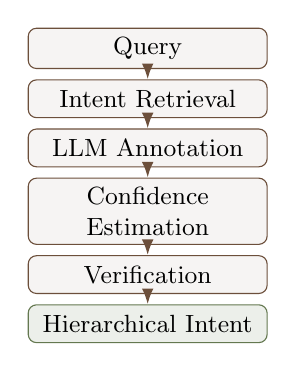
\begin{tikzpicture}[node distance=0.13cm]
\node[stage,minimum height=0.48cm] (query) {Query};
\node[stage,minimum height=0.48cm,below=of query] (retrieval) {Intent Retrieval};
\node[stage,minimum height=0.48cm,below=of retrieval] (annotation) {LLM Annotation};
\node[stage,minimum height=0.48cm,below=of annotation] (confidence) {Confidence Estimation};
\node[stage,minimum height=0.48cm,below=of confidence] (verification) {Verification};
\node[focus,minimum height=0.48cm,below=of verification] (hierarchy) {Hierarchical Intent};
\draw[link] (query) -- (retrieval);
\draw[link] (retrieval) -- (annotation);
\draw[link] (annotation) -- (confidence);
\draw[link] (confidence) -- (verification);
\draw[link] (verification) -- (hierarchy);
\end{tikzpicture}
\end{columns}
\end{frame}

\begin{frame}{Kết quả và giới hạn của nghiên cứu hiện tại}
\small
\begin{greenbox}{Thông điệp từ RVI-HIL}
Retrieval + verification hỗ trợ xây dựng hierarchical intent annotation trong Vietnamese e-commerce.
\end{greenbox}
\vspace{0.28cm}
\begin{columns}[T,onlytextwidth]
\column{0.31\textwidth}
\begin{uitbox}{1. Single-domain}
Chỉ đánh giá trên\par
\kw{Vietnamese e-commerce}.
\end{uitbox}
\column{0.31\textwidth}
\begin{uitbox}{2. Hierarchy theo domain}
Taxonomy được xây dựng riêng cho\par
\kw{e-commerce}.
\end{uitbox}
\column{0.31\textwidth}
\begin{uitbox}{3. Khả năng mở rộng}
Chưa kiểm tra quy trình trên\par
\kw{một domain khác}.
\end{uitbox}
\end{columns}
\vspace{0.32cm}
\begin{accentbox}{Câu hỏi nối tiếp}
\centering
\large Liệu quy trình hierarchical intent annotation có thể được mở rộng sang một domain hoàn toàn khác?
\end{accentbox}
\end{frame}

\section{2. Mở rộng sang BANKING77 và cấu trúc phân cấp}

\begin{frame}{Hướng mở rộng: từ e-commerce sang banking}
\centering
\begin{tikzpicture}
\node[stage,text width=4.1cm] (commerce) at (-3.4,1.2)
  {Vietnamese E-commerce\\\scriptsize Hasaki Q\&A};
\node[focus,text width=4.1cm] (banking) at (3.4,1.2)
  {Banking\\\scriptsize BANKING77};
\node[stage,text width=4.1cm] (existing) at (-3.4,-0.2)
  {Hierarchical intent annotation\\\scriptsize Nền tảng RVI-HIL};
\node[focus,text width=4.1cm] (construction) at (3.4,-0.2)
  {Flat $\rightarrow$ hierarchical taxonomy\\\scriptsize Phạm vi phase hiện tại};
\node[stage,text width=5.6cm] (shared) at (0,-1.9)
  {Hierarchical Intent\\\textbf{L1 $\rightarrow$ L2 $\rightarrow$ L3}};
\draw[link] (commerce) -- (existing);
\draw[link] (banking) -- (construction);
\draw[link] (existing.south) |- (shared.west);
\draw[link] (construction.south) |- (shared.east);
\end{tikzpicture}
\takeaway{Mục tiêu hiện tại: xây dựng taxonomy cho BANKING77 từ flat intent inventory.}
\vspace{0.1cm}
{\small Mở rộng miền dữ liệu; chưa đánh giá mô hình prediction hay chuyển giao ngôn ngữ.}
\end{frame}

\begin{frame}{BANKING77: một inventory gồm 77 flat intents}
\small
\begin{uitbox}{Dữ liệu gốc}
\kw{77 intent classes} trong banking; customer-service utterances bằng \kw{tiếng Anh}.\\
Nhãn gốc dạng \kw{flat}; không kèm hierarchy 3 tầng dùng trong nghiên cứu này.
\end{uitbox}
\vspace{0.08cm}
{\centering
\safeincludegraphics[trim=0 35 0 90,clip,width=\linewidth,height=0.38\textheight,keepaspectratio]{../prism-uploads/image_18.png}
\par\vspace{0.06cm}
{\scriptsize Mẫu dữ liệu: một utterance đi kèm nhãn intent \intent{card_arrival}.\par}
}
\takeaway{Flat Intent Inventory $\longrightarrow$ Hierarchical Intent Ontology}
\vspace{0.12cm}
{\tiny Nguồn: \href{https://aclanthology.org/2020.nlp4convai-1.5/}{Casanueva et al. (NLP4ConvAI, 2020), Efficient Intent Detection with Dual Sentence Encoders};
\href{https://github.com/PolyAI-LDN/task-specific-datasets/tree/master/banking_data}{PolyAI: banking\_data, categories.json}.}
\end{frame}

\begin{frame}{Bài báo giới thiệu bộ dữ liệu BANKING77}
\small
\textbf{Efficient Intent Detection with Dual Sentence Encoders}
\par\vspace{0.06cm}
{\scriptsize Casanueva et al. $\mid$ NLP4ConvAI 2020, tháng 7/2020 $\mid$ Association for Computational Linguistics}
\vspace{0.16cm}
\begin{columns}[T,onlytextwidth]
\column{0.57\textwidth}
\centering
\safeincludegraphics[trim=0 210 0 50,clip,width=\linewidth,height=0.48\textheight,keepaspectratio]{../prism-uploads/image_22.png}
\column{0.39\textwidth}
\begin{greenbox}{Đóng góp về dữ liệu}
\scriptsize
\begin{itemize}\setlength{\itemsep}{3pt}
\item Công bố \kw{BANKING77}: dữ liệu intent detection trong banking.
\item \textbf{13.083 mẫu có nhãn}, thuộc \textbf{77 intents}.
\item Customer-service utterances bằng \textbf{tiếng Anh}; nhãn intent dạng \textbf{flat}.
\end{itemize}
\end{greenbox}
\end{columns}
\vspace{0.13cm}
\centering
\begin{tikzpicture}
\node[stage,text width=4.5cm,minimum height=0.55cm] (original) at (-3.5,0)
  {\textbf{BANKING77 gốc (2020)}\\\scriptsize 77 flat intent labels};
\node[focus,text width=4.5cm,minimum height=0.55cm] (hierarchical) at (3.5,0)
  {\textbf{Hướng mở rộng hiện tại}\\\scriptsize Taxonomy L1 $\rightarrow$ L2 $\rightarrow$ L3};
\draw[link] (original) -- node[above,font=\tiny,align=center]{Bổ sung\\hierarchy} (hierarchical);
\end{tikzpicture}
\par\vspace{0.08cm}
{\scriptsize Bài báo cung cấp dữ liệu gốc; hierarchy 3 tầng là cấu trúc do nghiên cứu này đề xuất.}
\par\vspace{0.06cm}
{\tiny Nguồn: \href{https://aclanthology.org/2020.nlp4convai-1.5/}{Casanueva et al., NLP4ConvAI (2020), DOI: 10.18653/v1/2020.nlp4convai-1.5}.}
\end{frame}

\begin{frame}{Tại sao BANKING77 phù hợp?}
\small
\centering
\begin{columns}[T,onlytextwidth]
\column{0.48\textwidth}
\centering
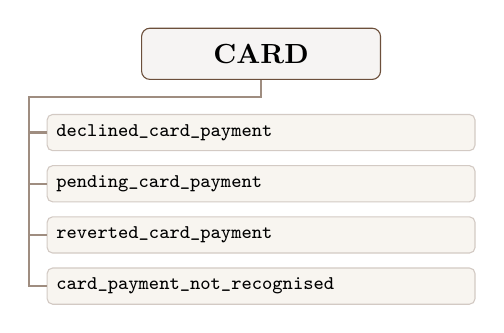
\begin{tikzpicture}
\node[stage,font=\bfseries] (card) at (0,0) {CARD};
\node[leaf,text width=5.2cm] (declined) at (0,-1) {\intent{declined_card_payment}};
\node[leaf,text width=5.2cm] (pending) at (0,-1.65) {\intent{pending_card_payment}};
\node[leaf,text width=5.2cm] (reverted) at (0,-2.3) {\intent{reverted_card_payment}};
\node[leaf,text width=5.2cm] (unrecognised) at (0,-2.95) {\intent{card_payment_not_recognised}};
\draw[branch] (card.south) -- (0,-0.55) -- (-2.95,-0.55) |- (declined.west);
\draw[branch] (-2.95,-0.55) |- (pending.west);
\draw[branch] (-2.95,-0.55) |- (reverted.west);
\draw[branch] (-2.95,-0.55) |- (unrecognised.west);
\end{tikzpicture}
\column{0.48\textwidth}
\centering
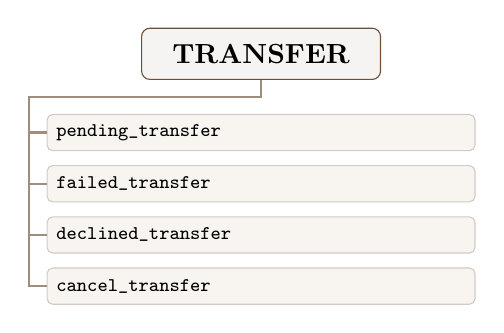
\begin{tikzpicture}
\node[stage,font=\bfseries] (transfer) at (0,0) {TRANSFER};
\node[leaf,text width=5.2cm] (pending) at (0,-1) {\intent{pending_transfer}};
\node[leaf,text width=5.2cm] (failed) at (0,-1.65) {\intent{failed_transfer}};
\node[leaf,text width=5.2cm] (declined) at (0,-2.3) {\intent{declined_transfer}};
\node[leaf,text width=5.2cm] (cancel) at (0,-2.95) {\intent{cancel_transfer}};
\draw[branch] (transfer.south) -- (0,-0.55) -- (-2.95,-0.55) |- (pending.west);
\draw[branch] (-2.95,-0.55) |- (failed.west);
\draw[branch] (-2.95,-0.55) |- (declined.west);
\draw[branch] (-2.95,-0.55) |- (cancel.west);
\end{tikzpicture}
\end{columns}
\vspace{0.12cm}
Cùng domain $\;\rightarrow\;$ gần nhau về intent family $\;\rightarrow\;$ khác ở fine-grained semantics.
\takeaway{Phù hợp để nghiên cứu tổ chức phân cấp các intent chi tiết.}
{\tiny Nhóm minh họa theo nhãn gốc; cần xác nhận bằng utterances và human validation.}
\end{frame}

\begin{frame}{Bài toán: Flat $\rightarrow$ Hierarchical Intent}
\small
\begin{columns}[c,onlytextwidth]
\column{0.43\textwidth}
\begin{uitbox}{Đầu vào: 77 flat intents}
\scriptsize
\intent{activate_my_card}\par
\intent{pending_card_payment}\par
\intent{failed_transfer}\par
\ldots\par
\intent{cash_withdrawal_charge}
\end{uitbox}
\column{0.08\textwidth}
\centering\Large\textcolor{accent}{$\Longrightarrow$}
\column{0.45\textwidth}
\centering
\begin{tikzpicture}[node distance=0.27cm]
\node[stage,text width=4.7cm] (levelone) {\textbf{L1} -- Nhóm dịch vụ chính};
\node[stage,text width=4.7cm,below=of levelone] (leveltwo) {\textbf{L2} -- Intent family};
\node[focus,text width=4.7cm,below=of leveltwo] (levelthree) {\textbf{L3} -- Original BANKING77 intent};
\draw[link] (levelone) -- (leveltwo);
\draw[link] (leveltwo) -- (levelthree);
\end{tikzpicture}
\end{columns}
\vspace{0.25cm}
\begin{accentbox}{Nguyên tắc bảo toàn}
\centering
\textbf{Không đổi semantic hoặc định danh của 77 intent gốc.}\\
Chỉ bổ sung các nhóm cha L1 / L2 và ánh xạ mỗi intent vào một path.
\end{accentbox}
{\scriptsize Quy ước: BANKING là root ngữ cảnh, nằm \textbf{ngoài} ba tầng L1--L2--L3.}
\end{frame}

\begin{frame}{Ví dụ Hierarchical BANKING77}

\vspace{0.22cm}
\begin{columns}[T,onlytextwidth]
\column{0.32\textwidth}
\centering
\intenttree{CARD (L1)}{PAYMENT (L2)}
{declined_card_payment,pending_card_payment,reverted_card_payment,card_payment_not_recognised}
\column{0.32\textwidth}
\centering
\intenttree{TRANSFER (L1)}{STATUS (L2)}
{pending_transfer,failed_transfer,declined_transfer}
\column{0.32\textwidth}
\centering
\intenttree{CASH\_WITHDRAWAL (L1)}{TRANSACTION\_PROBLEM (L2)}
{cash_withdrawal_charge,cash_withdrawal_not_recognised,wrong_amount_of_cash_received}
\end{columns}
\takeaway{L3 giữ nguyên các original intents; L1 / L2 là cấu trúc do nghiên cứu đề xuất.}
{\scriptsize Cần kiểm tra riêng: phí rút tiền có phù hợp với TRANSACTION\_PROBLEM hay cần nhóm phí?}
\end{frame}

\section{3. Xây dựng và kiểm chứng taxonomy}

\begin{frame}{Quy trình đề xuất để xây dựng taxonomy}
\small
\begin{columns}[T,onlytextwidth]
\column{0.55\textwidth}
\centering
\begin{tikzpicture}[node distance=0.14cm]
\node[stage,text width=5cm,minimum height=0.44cm] (inventory) {BANKING77: 77 flat labels};
\node[stage,text width=5cm,minimum height=0.44cm,below=of inventory] (examples) {Thu thập utterances đại diện};
\node[stage,text width=5cm,minimum height=0.44cm,below=of examples] (analysis) {Phân tích semantic};
\node[stage,text width=5cm,minimum height=0.44cm,below=of analysis] (grouping) {Đề xuất candidate grouping};
\node[stage,text width=5cm,minimum height=0.44cm,below=of grouping] (construction) {Xây dựng hierarchy L1 / L2};
\node[stage,text width=5cm,minimum height=0.44cm,below=of construction] (verification) {Human verification};
\node[focus,text width=5cm,minimum height=0.44cm,below=of verification] (final) {Taxonomy 3 tầng sau adjudication};
\draw[link] (inventory) -- (examples);
\draw[link] (examples) -- (analysis);
\draw[link] (analysis) -- (grouping);
\draw[link] (grouping) -- (construction);
\draw[link] (construction) -- (verification);
\draw[link] (verification) -- (final);
\draw[link,draw=accent] (verification.east) -- ++(0.55,0)
  |- node[pos=0.25,right,font=\tiny,align=left]{Sửa nhóm\\khi bất đồng} (grouping.east);
\end{tikzpicture}
\column{0.41\textwidth}
\begin{greenbox}{Tiêu chí cho mỗi grouping}
\begin{itemize}\setlength{\itemsep}{4pt}
\item Semantic coherence.
\item Quan hệ parent--child hợp lý.
\item Siblings đủ tương đồng.
\item Siblings vẫn phân biệt được.
\item Coverage đủ 77 intents.
\item Không có orphan intent.
\end{itemize}
\end{greenbox}
\end{columns}
\takeaway{Research-constructed hierarchical ontology for BANKING77}
{\scriptsize Không phải taxonomy chính thức của bộ dữ liệu BANKING77.}
\end{frame}

\begin{frame}{Taxonomy validation: cấu trúc và ngữ nghĩa}
\small
\begin{columns}[T,onlytextwidth]
\column{0.48\textwidth}
\begin{uitbox}{Kiểm tra theo tầng}
\textbf{L1:} cùng nhóm dịch vụ chính?\par\vspace{0.12cm}
\textbf{L2:} cùng intent family?\par\vspace{0.12cm}
\textbf{L3 siblings:} đủ gần để cùng nhóm, nhưng đủ khác để phân biệt?
\end{uitbox}
\vspace{0.1cm}
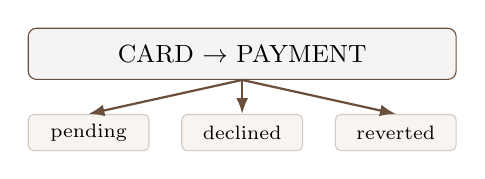
\begin{tikzpicture}
\node[stage,text width=5.2cm] (family) {CARD $\rightarrow$ PAYMENT};
\node[leaf,text width=1.3cm,align=center] (pending) at (-1.95,-1) {pending};
\node[leaf,text width=1.3cm,align=center] (declined) at (0,-1) {declined};
\node[leaf,text width=1.3cm,align=center] (reverted) at (1.95,-1) {reverted};
\draw[link] (family.south) -- (pending.north);
\draw[link] (family.south) -- (declined.north);
\draw[link] (family.south) -- (reverted.north);
\end{tikzpicture}
\column{0.48\textwidth}
\begin{greenbox}{Human validation -- kế hoạch}
\begin{enumerate}\setlength{\itemsep}{4pt}
\item \textbf{3--5 annotators / experts}: xem định nghĩa và utterances đại diện.
\item Gán độc lập L1 / L2 cho cùng 77 intents theo guideline chung.
\item Báo cáo agreement riêng theo tầng; \textbf{Fleiss' $\kappa$} cho nhiều người, \textbf{Cohen's $\kappa$} cho hai người.
\item Adjudication khi bất đồng; lưu lý do và cập nhật taxonomy.
\end{enumerate}
\end{greenbox}
\end{columns}
\takeaway{Agreement hỗ trợ đánh giá; không thay thế kiểm tra semantic và adjudication.}
\end{frame}

\begin{frame}{Kết quả mong muốn của phase hiện tại}
\centering
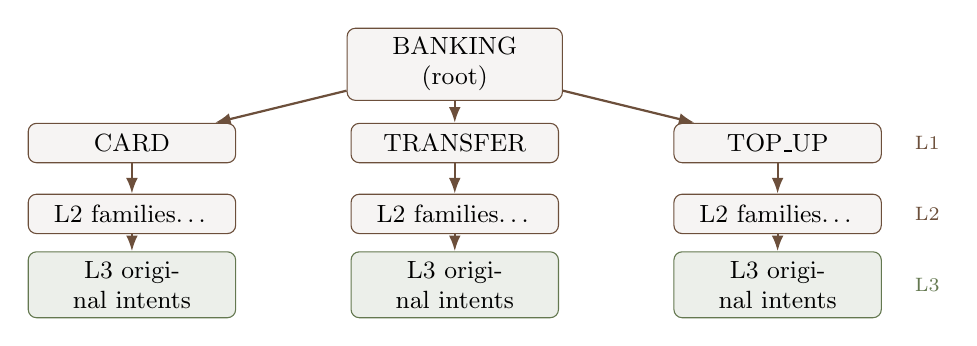
\begin{tikzpicture}
\node[stage,text width=2.5cm,minimum height=0.5cm] (root) at (0,0) {BANKING (root)};
\node[stage,text width=2.4cm,minimum height=0.5cm] (card) at (-4.1,-1) {CARD};
\node[stage,text width=2.4cm,minimum height=0.5cm] (transfer) at (0,-1) {TRANSFER};
\node[stage,text width=2.4cm,minimum height=0.5cm] (topup) at (4.1,-1) {TOP\_UP};
\node[stage,text width=2.4cm,minimum height=0.5cm] (cardfamily) at (-4.1,-1.9) {L2 families\ldots};
\node[stage,text width=2.4cm,minimum height=0.5cm] (transferfamily) at (0,-1.9) {L2 families\ldots};
\node[stage,text width=2.4cm,minimum height=0.5cm] (topupfamily) at (4.1,-1.9) {L2 families\ldots};
\node[focus,text width=2.4cm,minimum height=0.5cm] (cardintent) at (-4.1,-2.8) {L3 original intents};
\node[focus,text width=2.4cm,minimum height=0.5cm] (transferintent) at (0,-2.8) {L3 original intents};
\node[focus,text width=2.4cm,minimum height=0.5cm] (topupintent) at (4.1,-2.8) {L3 original intents};
\draw[link] (root) -- (card);
\draw[link] (root) -- (transfer);
\draw[link] (root) -- (topup);
\draw[link] (card) -- (cardfamily);
\draw[link] (transfer) -- (transferfamily);
\draw[link] (topup) -- (topupfamily);
\draw[link] (cardfamily) -- (cardintent);
\draw[link] (transferfamily) -- (transferintent);
\draw[link] (topupfamily) -- (topupintent);
\node[font=\scriptsize,text=uitblue] at (6,-1) {L1};
\node[font=\scriptsize,text=uitblue] at (6,-1.9) {L2};
\node[font=\scriptsize,text=greenteal] at (6,-2.8) {L3};
\end{tikzpicture}
\vspace{0.12cm}
\begin{columns}[T,onlytextwidth]
\column{0.48\textwidth}
\begin{uitbox}{Tiêu chí hoàn thành}
\small 77/77 intents giữ nguyên; mỗi intent có \textbf{một path L1 $\rightarrow$ L2 $\rightarrow$ L3}.
\end{uitbox}
\column{0.48\textwidth}
\begin{greenbox}{Sản phẩm bàn giao}
\small Bộ datasets có đầy đủ L1,L2,L3 của các câu query
\end{greenbox}
\end{columns}
\vspace{0.08cm}
{\scriptsize Sơ đồ minh họa một phần; số nhóm và grouping cuối cùng phụ thuộc validation.}
\end{frame}

\section{4. Hướng phát triển tiếp theo}

\begin{frame}{Bước tiếp theo: Hierarchical Intent Prediction}
\centering
\begin{tikzpicture}
\node[stage,text width=3.5cm,minimum height=1cm] (previous) at (-4.5,0)
  {\textbf{RVI-HIL}\\\scriptsize Hierarchical intent annotation};
\node[focus,text width=3.5cm,minimum height=1cm] (current) at (0,0)
  {\textbf{Phase hiện tại}\\\scriptsize Flat $\rightarrow$ Hierarchical BANKING77};
\node[future,text width=3.5cm,minimum height=1cm] (next) at (4.5,0)
  {\textbf{Phase tiếp theo}\\\scriptsize Hierarchical intent prediction};
\draw[link] (previous) -- (current);
\draw[link] (current) -- (next);
\end{tikzpicture}
\vspace{0.32cm}
\begin{columns}[T,onlytextwidth]
\column{0.47\textwidth}
\begin{uitbox}{Bài toán tương lai}
\centering\small
Query $\rightarrow$ Predict L1 $\rightarrow$ Predict L2 $\rightarrow$ Predict L3
\end{uitbox}
\column{0.49\textwidth}
\begin{greenbox}{Các hướng sẽ khảo sát}
\small
Flat vs. hierarchical classification; parent--child conditioning; sibling-aware learning; fine-grained prediction.
\end{greenbox}
\end{columns}
\vspace{0.16cm}
\end{frame}

\section{5. Hiện trạng Intent Classification tại Việt Nam}

\begin{frame}{Hiện trạng tại Việt Nam: nghiên cứu và ứng dụng}
\small
\begin{columns}[T,onlytextwidth]
\column{0.48\textwidth}
\begin{uitbox}{Tran \& Luong (2020)}
\scriptsize\textsl{Understanding what the users say in chatbots: A case study for the Vietnamese language}
\par\vspace{0.12cm}
\small Vietnamese e-commerce chatbot.\\
\kw{Flat Intent Classification}.\\
F1 = \textbf{82.32\%} trên dữ liệu đánh giá của bài báo.
\end{uitbox}
\column{0.48\textwidth}
\begin{uitbox}{Luong Thai Le (2020)}
\scriptsize\textsl{Intent Domain Identification Using Deep Learning Model}
\par\vspace{0.12cm}
\small Phân loại miền ý định cho câu hỏi tiếng Việt.\\
\kw{Intent Domain Classification}.\\
Mô hình dựa trên \textbf{CNN}.
\end{uitbox}
\end{columns}
\vspace{0.2cm}
\begin{greenbox}{Ứng dụng thực tế: Hieu Tran -- MoMo (2022)}
\scriptsize\textsl{How We Build a Conversational AI Chatbot at MoMo}
\par\vspace{0.1cm}
\small Có thiết kế \kw{hierarchical intent classification}:\quad
\textbf{General Intent $\rightarrow$ Specific Intent}.\\
Bài viết kỹ thuật công nghiệp; không phải bài báo công bố benchmark học thuật.
\end{greenbox}
\vspace{0.08cm}
{\tiny Nguồn: \href{https://js.vnu.edu.vn/CS/article/view/4202}{Tran \& Luong, VNU JCSCE (2020)};
\href{https://proceeding.conferenceworld.in/ICSTM-XVI/5.pdf}{Le, ICSTM-XVI (2020)};
\href{https://ai.momo.vn/blog/how-we-build-a-conversational-ai-chatbot-at-momo}{Hieu Tran, MoMo AI (2022)}.}
\end{frame}

\begin{frame}{Research gap: ý định phân cấp chi tiết cho tiếng Việt}
\small
\centering
\begin{tikzpicture}
\node[stage,text width=5.4cm] (existing) at (-3.4,0)
  {\textbf{Hai nghiên cứu học thuật vừa nêu}\\
   Query $\rightarrow$ Intent / Intent Domain};
\node[focus,text width=5.4cm] (target) at (3.4,0)
  {\textbf{Bài toán hướng tới}\\
   Vietnamese Query $\rightarrow$ L1 $\rightarrow$ L2 $\rightarrow$ L3};
\draw[link,draw=accent] (existing) -- (target);
\end{tikzpicture}
\vspace{0.22cm}
\begin{columns}[T,onlytextwidth]
\column{0.48\textwidth}
\begin{uitbox}{Hiện trạng khảo sát}
\scriptsize
Hai bài học thuật: \kw{flat intent} hoặc \kw{intent-domain}.\\
Bài viết MoMo: hierarchy 2 tầng (general $\rightarrow$ specific), không có benchmark công bố.\\
VNTC: phân loại chủ đề tin tức, không phải fine-grained intent.
\end{uitbox}
\column{0.48\textwidth}
\begin{greenbox}{Khoảng trống}
\scriptsize
Chưa có đánh giá học thuật đầy đủ cho fine-grained hierarchical intent \textbf{L1 $\rightarrow$ L2 $\rightarrow$ L3} trên tiếng Việt, đặc biệt khi mở rộng sang domain mới.
\end{greenbox}
\end{columns}
\vspace{0.14cm}
\begin{accentbox}{Định hướng nghiên cứu}
\centering\small
\textbf{Fine-grained Hierarchical Intent Classification for Vietnamese remains underexplored.}\\[0.1cm]
Flat Intent $\rightarrow$ Hierarchical Taxonomy $\rightarrow$ Hierarchical Prediction
\end{accentbox}
{\tiny Nhận định trong phạm vi tài liệu khảo sát; không khẳng định chưa có nghiên cứu khác.
Nguồn dữ liệu topic/news: \href{https://github.com/duyvuleo/VNTC}{VNTC -- Vietnamese News Text Classification}.}
\end{frame}

\end{document}
